
\chapter*{Chapter 6}
\markboth{Sprint 4 : Feedback \& Reviews}{Sprint 4 : Feedback \& Reviews} %pour afficher l'entete
 \addcontentsline{toc}{chapter}{6 Sprint 4 : Feedback \& Reviews}


\setcounter{chapter}{6}
\setcounter{section}{0}
\setcounter{table}{0} 
\setcounter{figure}{0} 


\etocsettocstyle{\subsection*{Plan}}{}
\vspace{0.25cm}

\setcounter{tocdepth}{1}
\headrule{
\vspace{0.5cm}

\begin{center}
    \textsc{\textbf {\Huge Sprint 4 : Feedback \& Reviews}} 
\end{center}
}
\headrule


\localtableofcontents
\newpage

\section*{Introduction}
Following the cartography module, this chapter details the development of the "Feedback \& Reviews" module, the last major feature of our app. This module allows users to share their experiences and rate the app, providing us with essential insights to enhance user satisfaction and application performance.

\section{Sprint 2 Backlog}

The sprint backlog is a detailed list of tasks and user stories selected for completion within the current sprint, guiding the development team's work towards achieving the sprint goal. It serves as a dynamic, prioritized plan that evolves as the team progresses and new information emerges.
The table below describes the backlog of the second sprint :



\begin{table}[H]
    % \centering
    \renewcommand{\arraystretch}{1.2}
    \setlength{\belowcaptionskip}{0.25cm}
 
   \begin{tabular}{|p{0.05\textwidth}|p{0.2\textwidth}|p{0.34\textwidth}|p{0.34\textwidth}|}
   \hline
   \textbf{ID}  &  \textbf{User Story } & \textbf{Description} & \textbf{Task} \\ \hline


   
   \begin{center}
       \textbf{1}
   \end{center} & \begin{center}
       As a user, I want submit a feedback or report an issue
   \end{center} &
   \begin{center}
   The user can send feedback or report an issue that bother his experience.
   \end{center} &
       \begin{itemize}[left=0pt, label={\textbf{\Huge .}}]
       % \renewcommand\labelitemi{\textbf{\Huge .}}
            \item Develop the module's backend 
            \item Develop the user interface 
        \end{itemize} \\ \hline
   \begin{center}
       \textbf{2}
   \end{center} & \begin{center}
       As a  user, I want to track the reported issues 
   \end{center} &
   \begin{center}
       
  The  user can consult his sent messages and read the IT team responses.\end{center}
  & 
       \begin{itemize}[left=0pt, label={\textbf{\Huge .}}]
            \item Develop the module's backend 
            \item Develop the user interface 
        \end{itemize} \\ \hline
\end{tabular}
       \caption{Sprint 2 Backlog}
        \label{tab:my_label}
\end{table}
\newpage

\section{Sprint 4 use case diagram}

The figure below showcases the use case diagram for this sprint the involved actors and the expected functionalities  from our application.

\begin{figure}[H]
    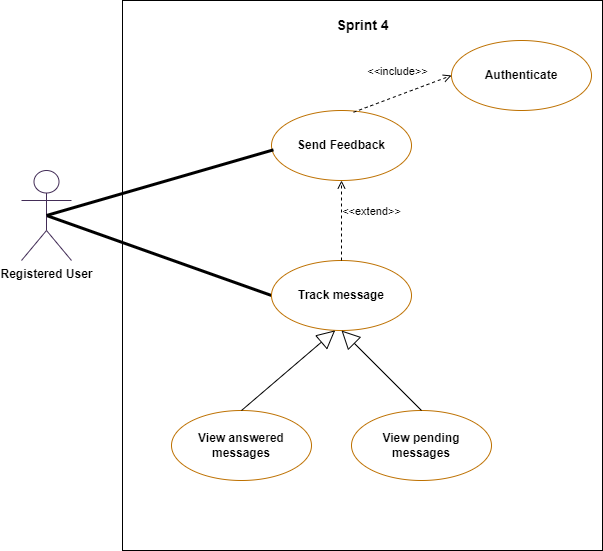
\includegraphics[width=0.98\textwidth]{images/sprint4/Sprint4UC.png}
     \caption{Sprint 4 Use Case Diagram}
    \label{fig:enter-label}
    
\end{figure}

\newpage
\section{User story n°1 : Send Feedback}
\textbf{\underline{Text description of the “Send Feedback” use case}}

\vspace{0.25cm}
We detail through this table the use case “Send Feedback” :

\begin{table}[H]
    % \centering
    \renewcommand{\arraystretch}{1.5}
    
   \begin{tabular}{|p{0.25\textwidth}|p{0.68\textwidth}|}
   \hline
     
        \textbf{Use Case} & Send Feedback  \\   \hline
        
        \textbf{Actor(s) } &  Authenticated user   \\   \hline
        \textbf{Pre-condition} & 
           The User request the feedback page.
         
        \\  \hline
        \textbf{Post-condition} & None \\   \hline


                \textbf{Principal scenario} &
                \begin{enumerate}[left=0pt]
                    \item The user gives a rating.
                    \item The user enters the report type.
                    \item The user types his message .
                    \item The system adds the review .
                    \item The system displays a success message .
                
                    \end{enumerate}  \\   \hline

                     \textbf{Alternative\newline scenario} & 
            If the user has an empty field a warning message appears.
        \\   \hline
       
\end{tabular}

     \caption{Text Description Of The “Send Feedback” Use Case}
    \label{tab:my_label}
    
\end{table}

\newpage

\subsection{Sequence Diagram <<Send feedback>> }



\begin{figure}[H]
   
    
    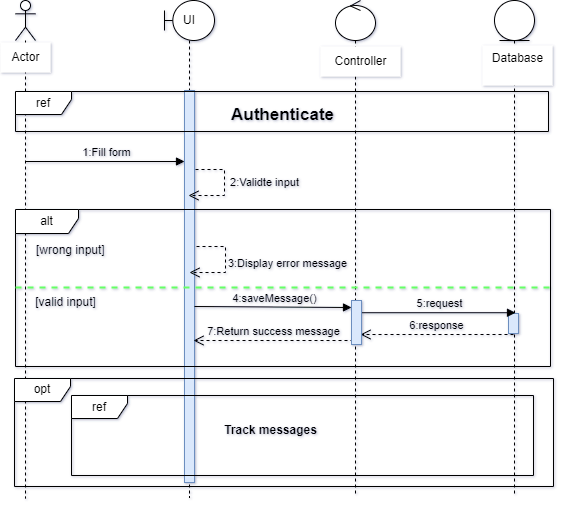
\includegraphics[width=0.98\textwidth]{images/sprint4/feedbackSeq.png}
    \caption{“Send Feedback” Sequence Diagram}
    \label{fig:enter-label}
    
\end{figure}
\newpage
\subsection{Sprint 2 Class Diagram}
\begin{figure}[H]
   
    
    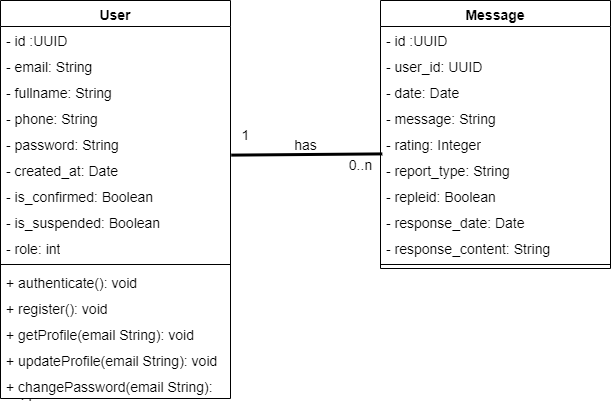
\includegraphics[width=0.98\textwidth]{images/sprint4/Sprint4ClassDiag.png}
    \caption{Sprint 2 Class Diagram}
    \label{fig:enter-label}
    
\end{figure}
\newpage
\subsection{Realization}
In the section we will explore the final user interfaces related to the user story n°1 : "Send Feedback" in a sequential order :
\begin{figure}[H]
\begin{minipage}{0.32\textwidth}
    \centering
    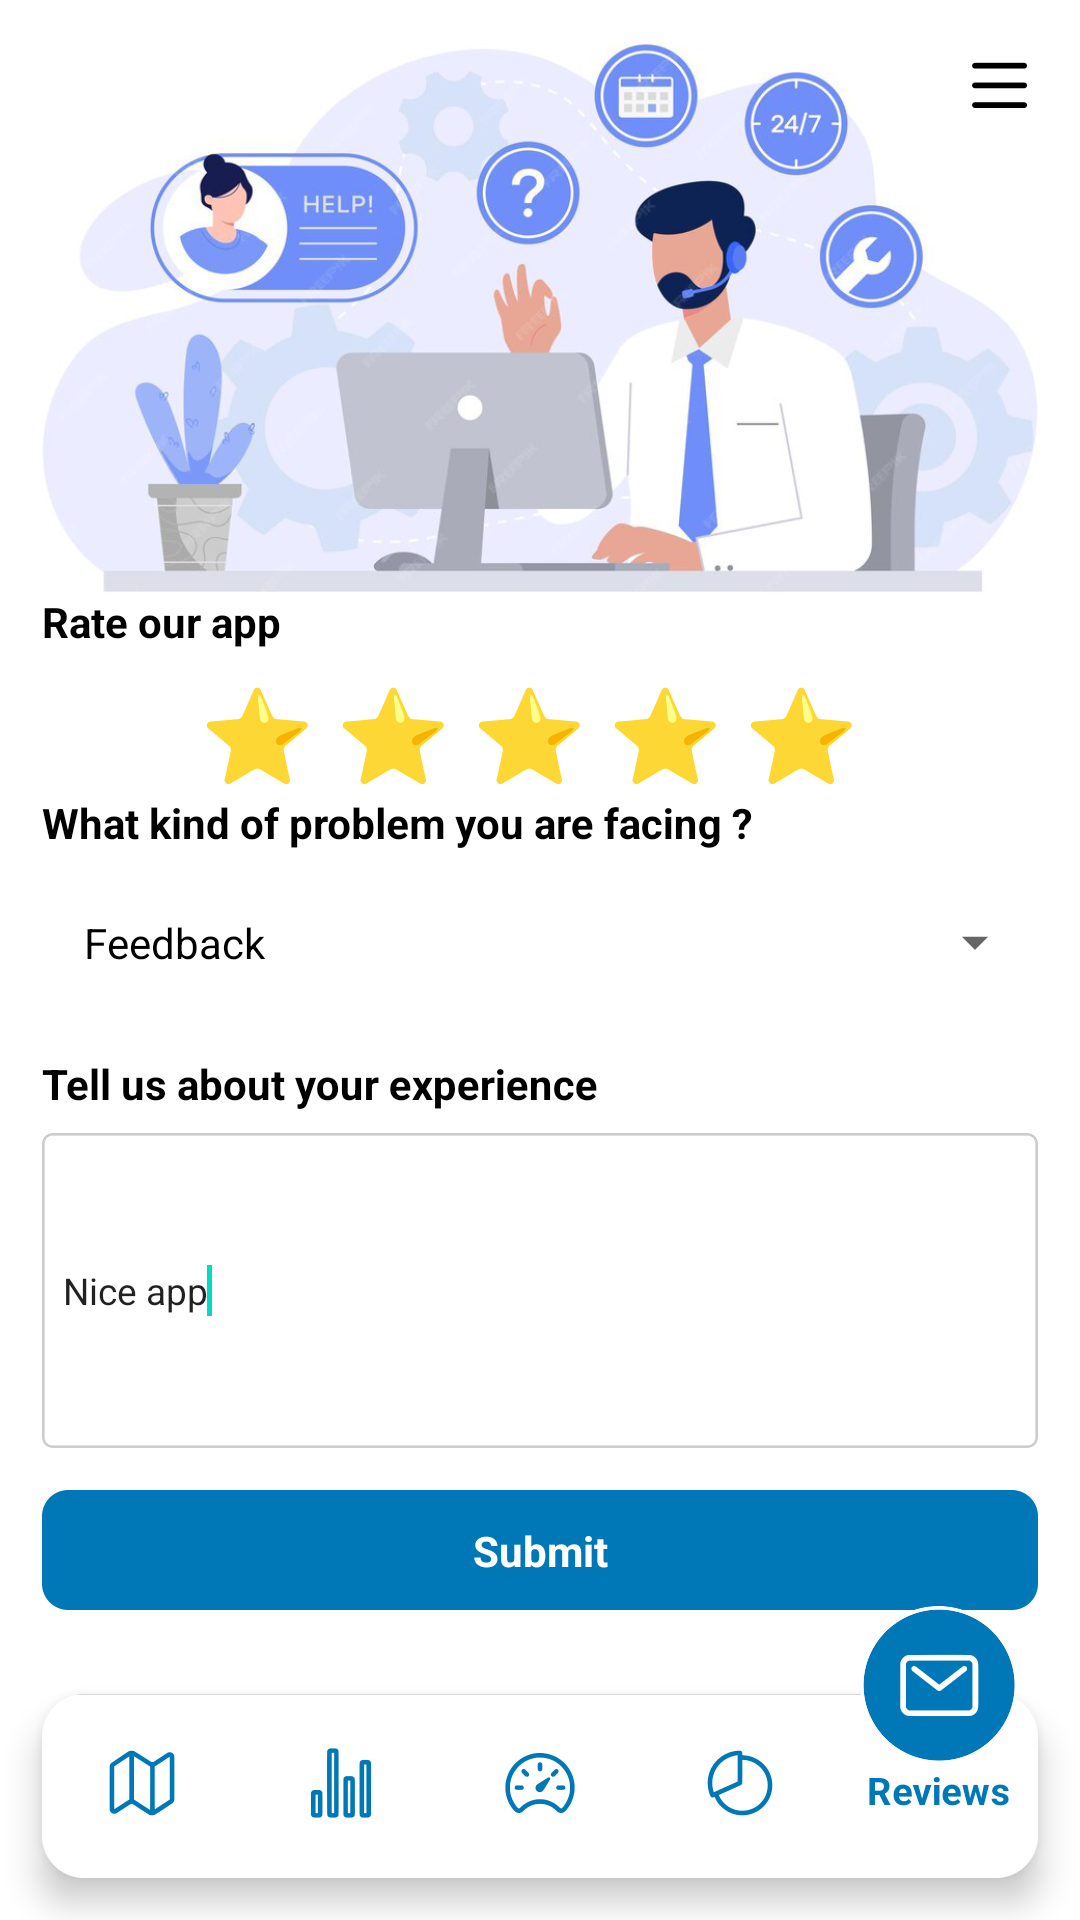
\includegraphics[width=\linewidth]{images/sprint4/feedBackModule (6).png}
    \label{fig:login-form-filled}
\end{minipage}\hfill
\begin{minipage}{0.32\textwidth}
    \centering
    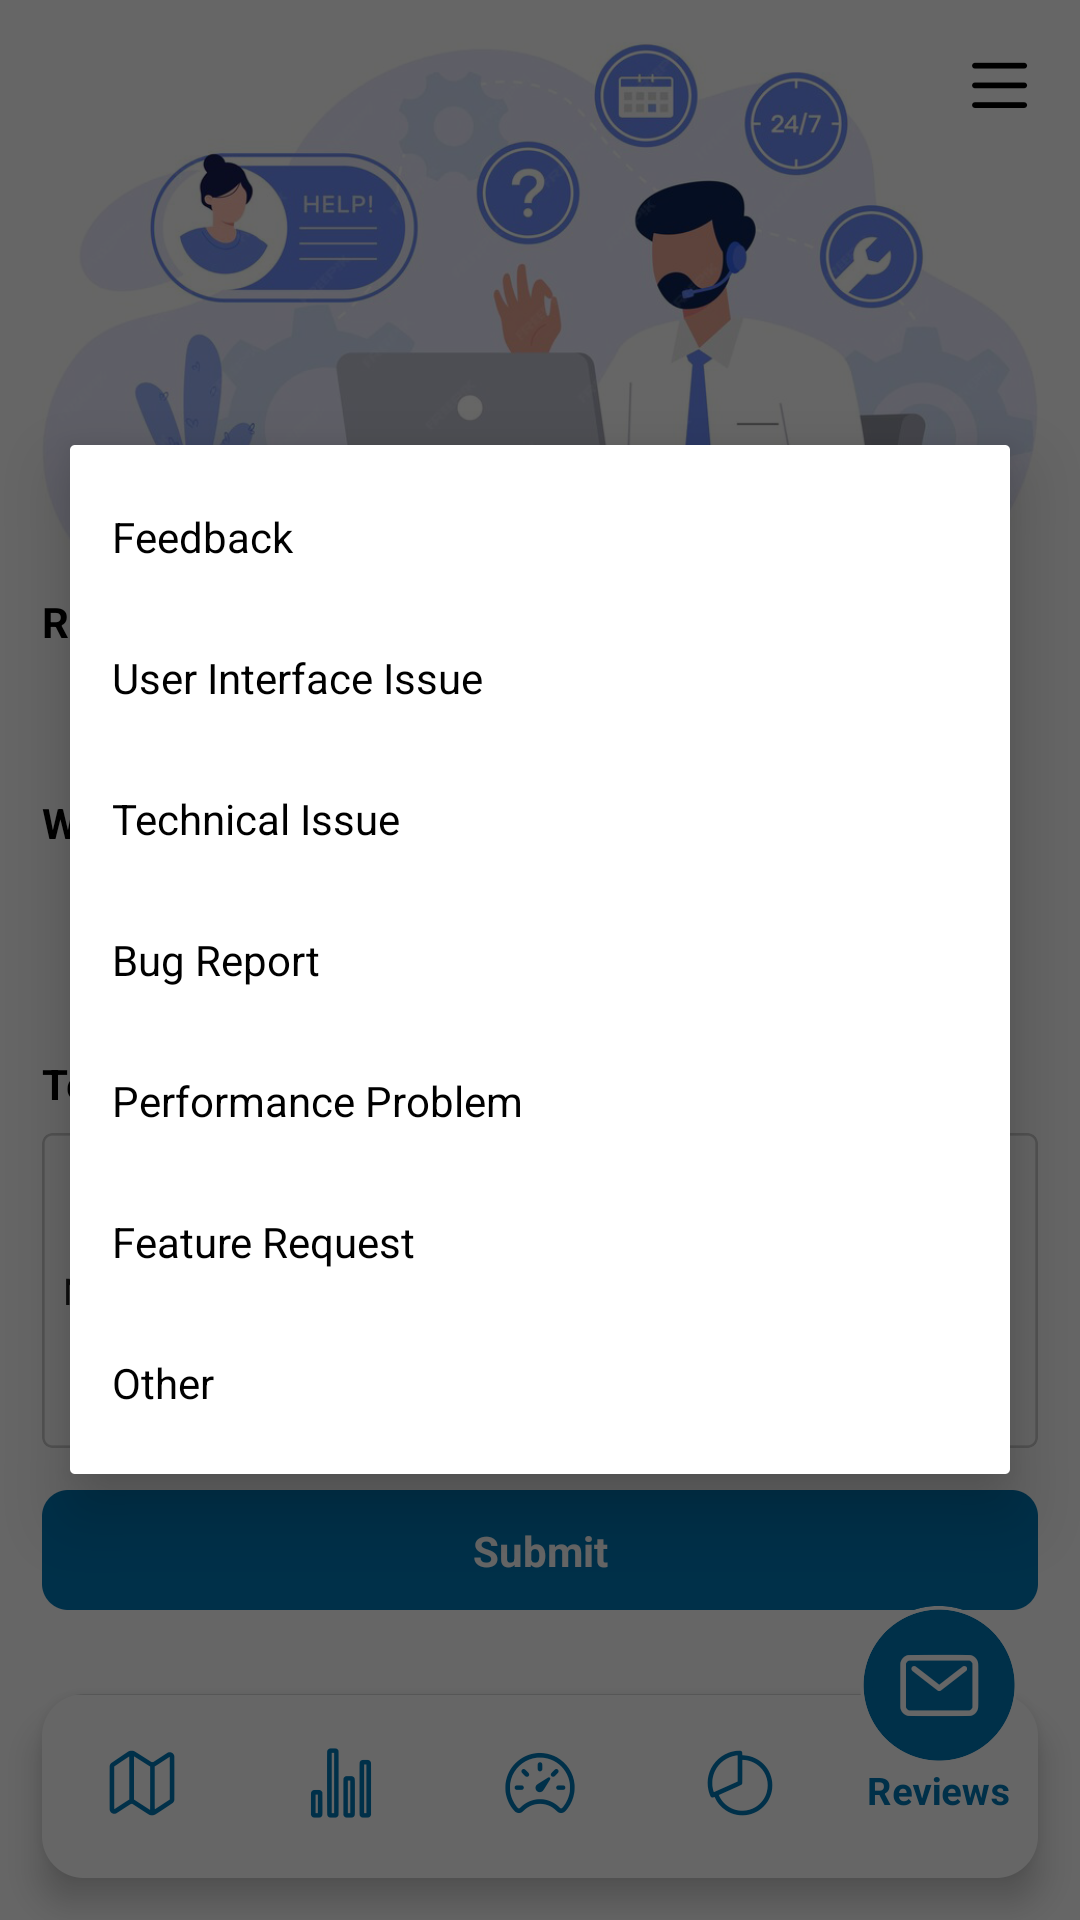
\includegraphics[width=\linewidth]{images/sprint4/feedBackModule (5).png}
    \label{fig:login-form}
\end{minipage}\hfill
    \caption{Feedback Screen}
\end{figure}
\newpage
\section{User story n°2 : Track messages}

\textbf{\underline{Text description of the “Track messages”use case:}}

\vspace{0.25cm}

We detail through this table the use case “Track messages” :

\begin{table}[H]
    % \centering
    \renewcommand{\arraystretch}{1.5}
    
   \begin{tabular}{|p{0.25\textwidth}|p{0.68\textwidth}|}
   \hline
     
        \textbf{Use Case} & View Reports  \\   \hline
        
        \textbf{Actor(s) } & Authenticated User  \\   \hline
        \textbf{Pre-condition} & The user requests the reports screen \\   \hline
        \textbf{Post-condition} & None  \\   \hline
                \textbf{Principal scenario} & 
                \begin{enumerate}
                    \item The user enters the reports screen.
                    \item The system retrieve the data related to the user .
                    \item The user interacts with the default charts.
                    \item The request an other chart.
                    \item The system extract the needed values and display the requested chart.
                \end{enumerate}  \\   \hline
        
        \textbf{Alternative\newline scenario} & 
        \begin{center}
            
        If user has not save any test yet a user friendly message appears.
        \end{center}
         \\   \hline
\end{tabular}
     \caption{Text Description Of The “Track messages” Use Case}
    \label{tab:my_label}
\end{table}


\newpage

\subsection{Sequence Diagram<<Track messages>> }
Below, we present the sequence diagrams for each use case mentioned above.

\begin{figure}[H]
   
    
    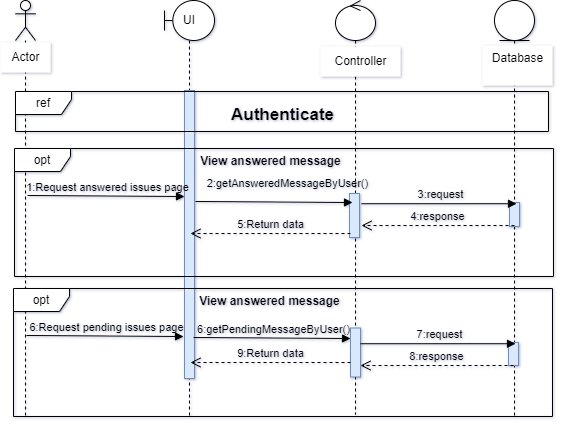
\includegraphics[width=0.98\textwidth]{images/sprint4/trackMsgSeq.png}
    \caption{News Feed - View News sequence diagram}
    \label{fig:enter-label}
    
\end{figure}
\newpage
\subsection{Realization}
In this section we will showcase the final outcome of the second user story of this sprint :
\begin{figure}[H]
\begin{minipage}{0.35\textwidth}
    \centering
    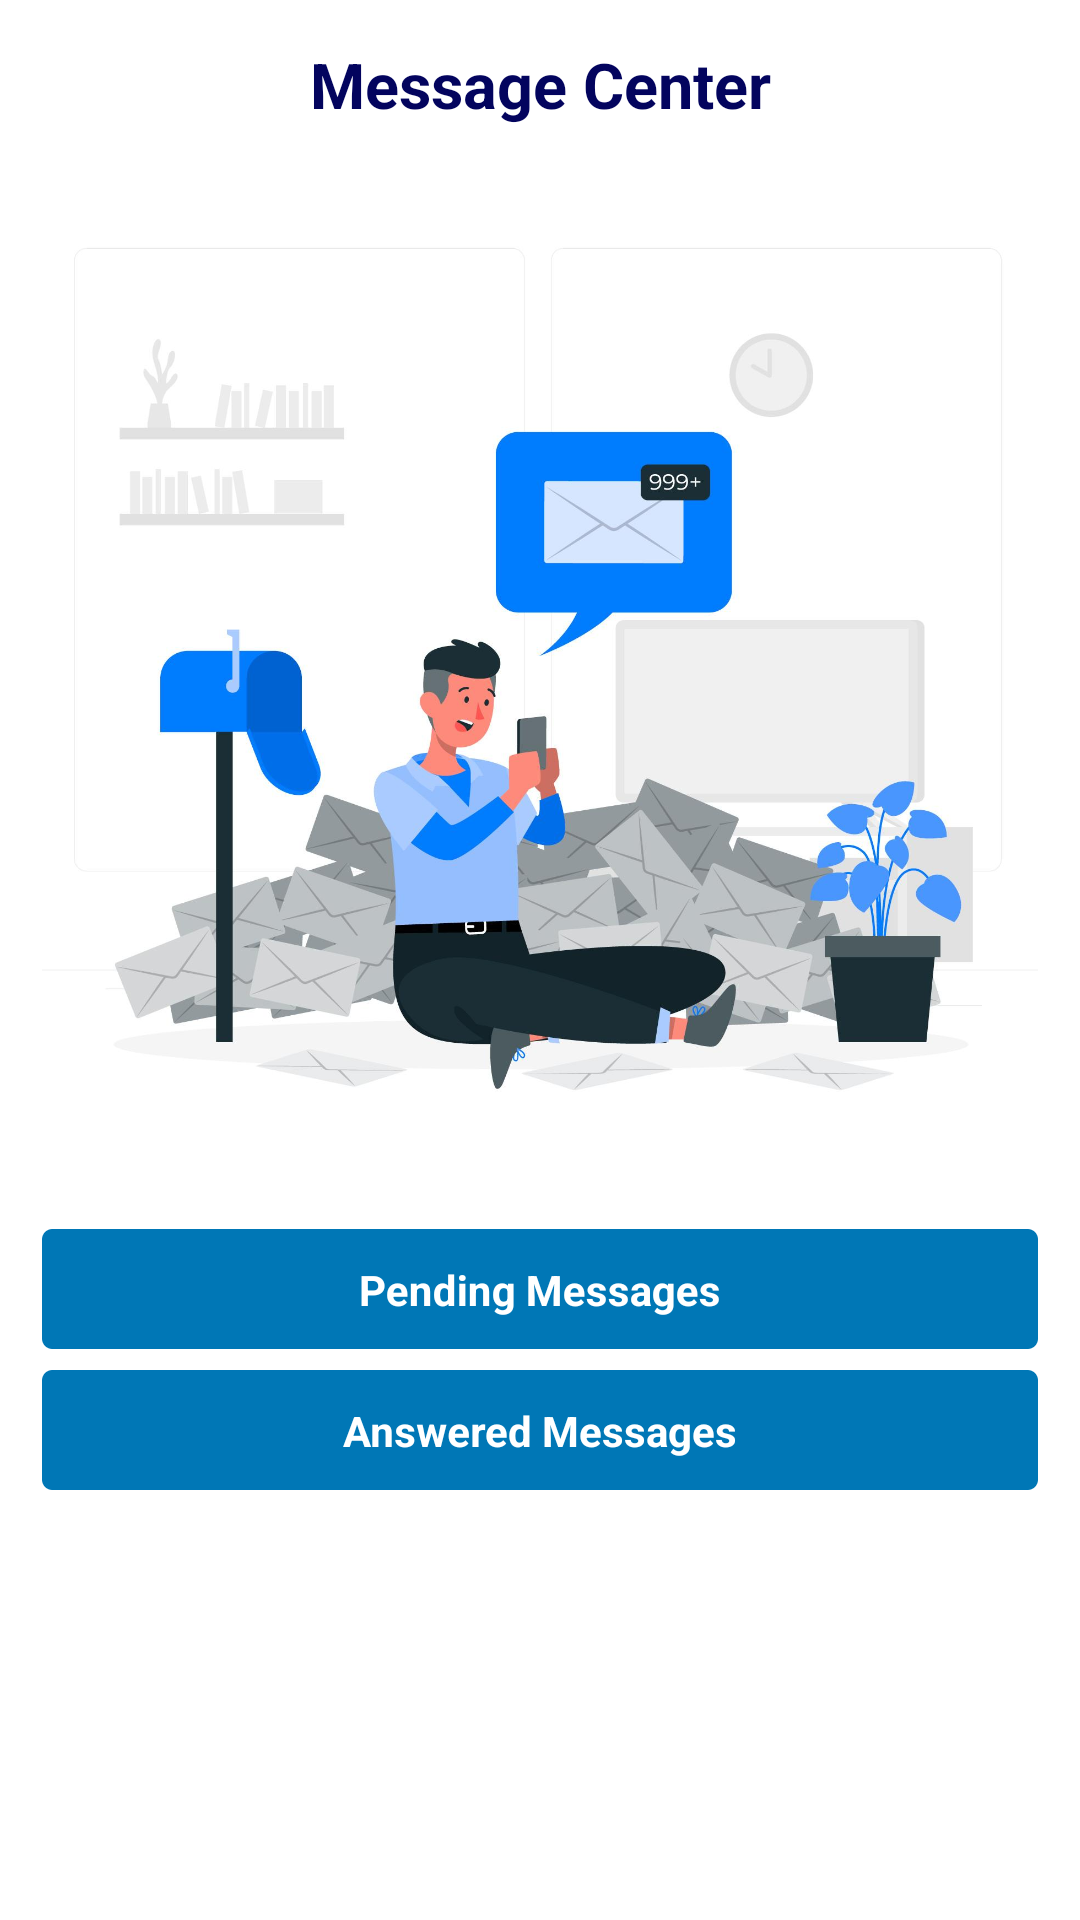
\includegraphics[width=\linewidth]{images/sprint4/feedBackModule (7).png}
    \label{fig:login-form-filled}
\end{minipage}\hfill
\begin{minipage}{0.35\textwidth}
    \centering
    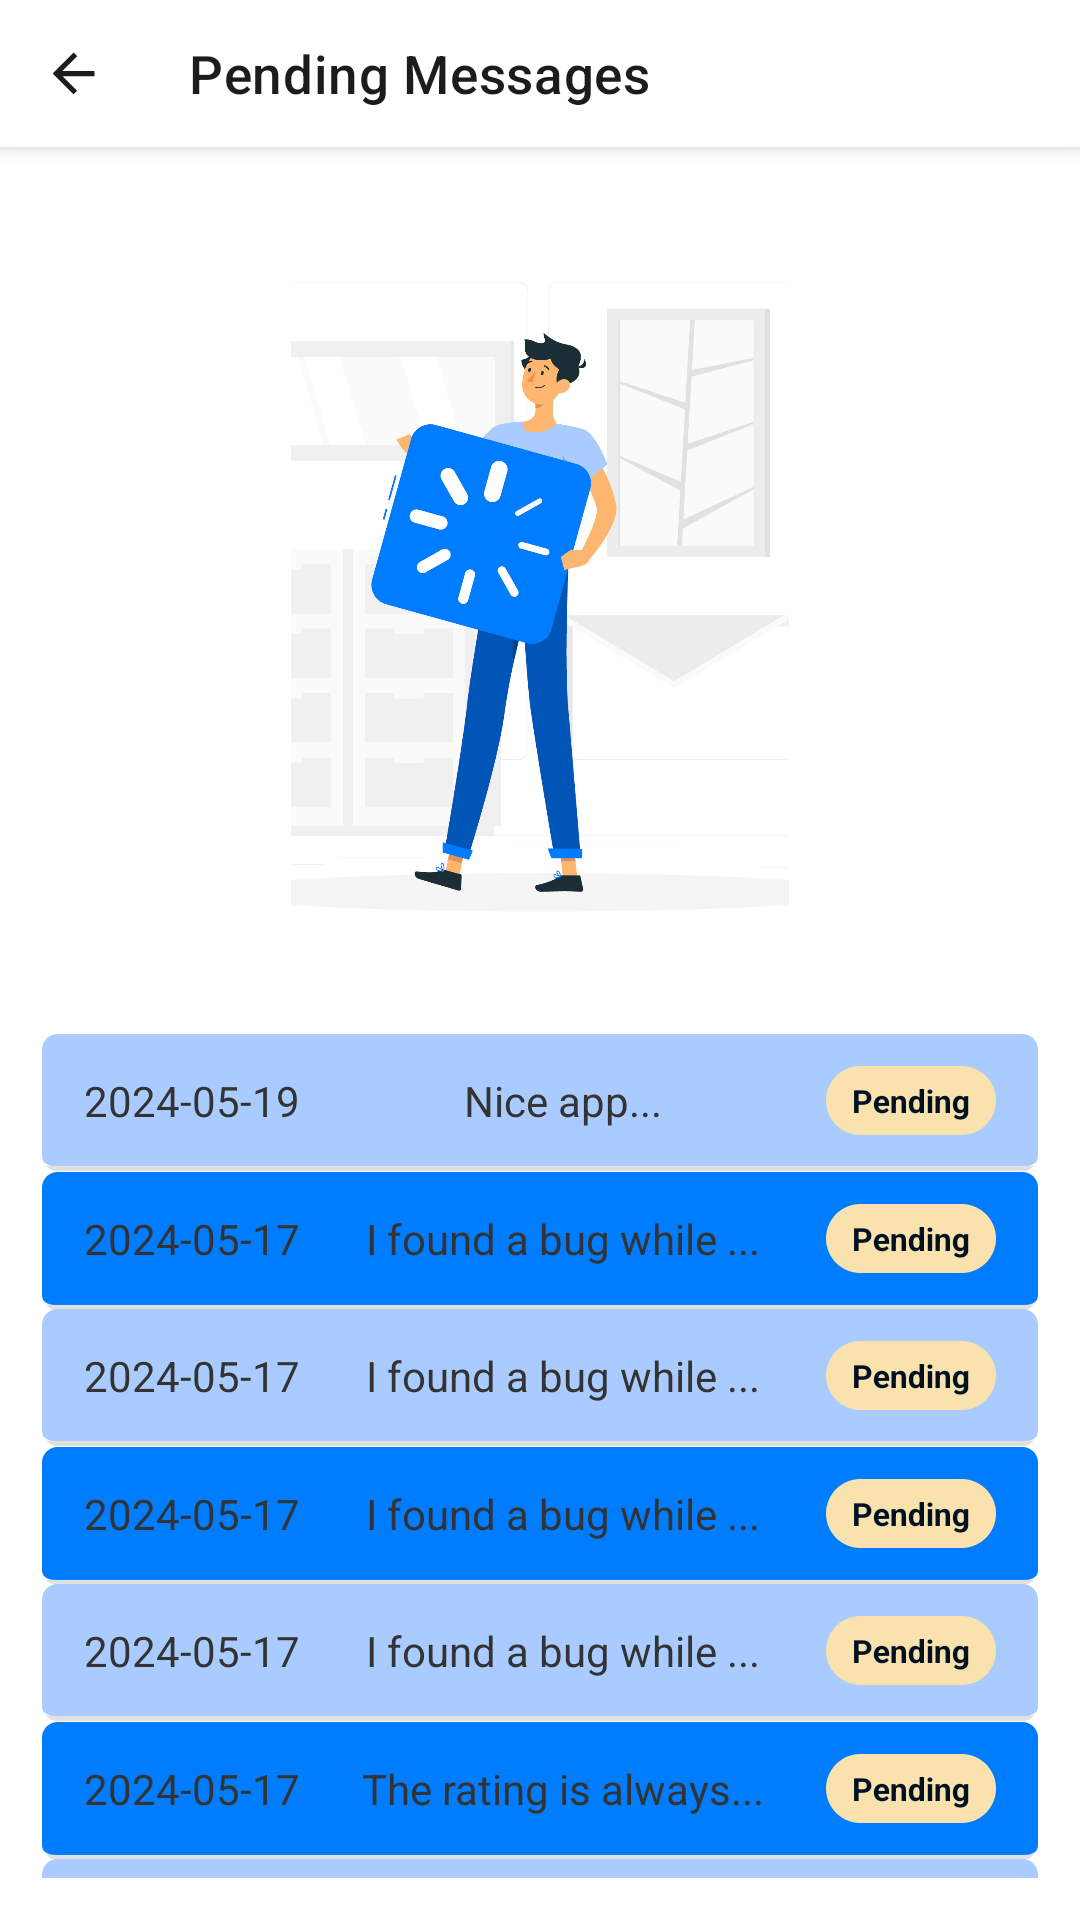
\includegraphics[width=\linewidth]{images/sprint4/feedBackModule (2).png}
    % \caption{Forget Password Sequence Diagram Part 1}
    \label{fig:login-form}
\end{minipage}\hfill
    % \caption{Reports Screen}
\end{figure}
\begin{figure}[H]
\begin{minipage}{0.35\textwidth}
    \centering
    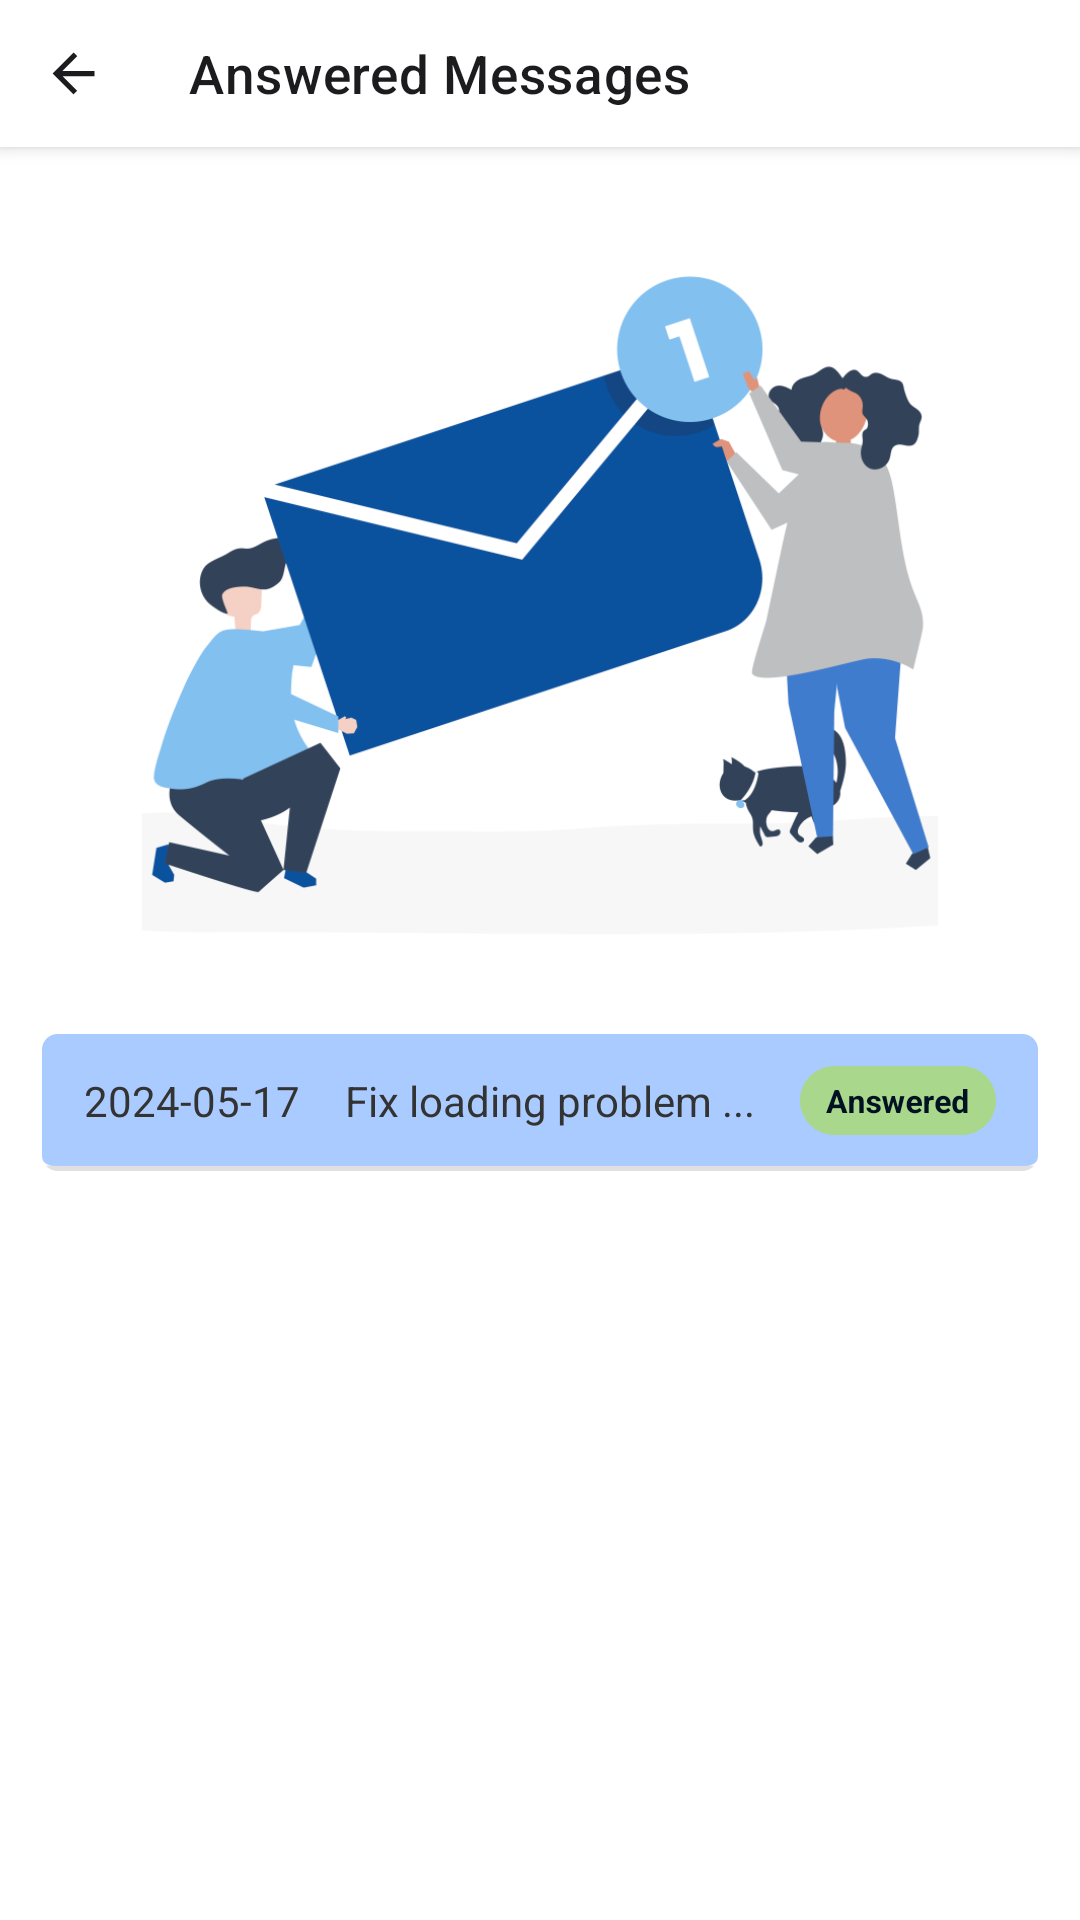
\includegraphics[width=\linewidth]{images/sprint4/feedBackModule (4).png}
    \label{fig:login-form-filled}
\end{minipage}\hfill
\begin{minipage}{0.35\textwidth}
    \centering
    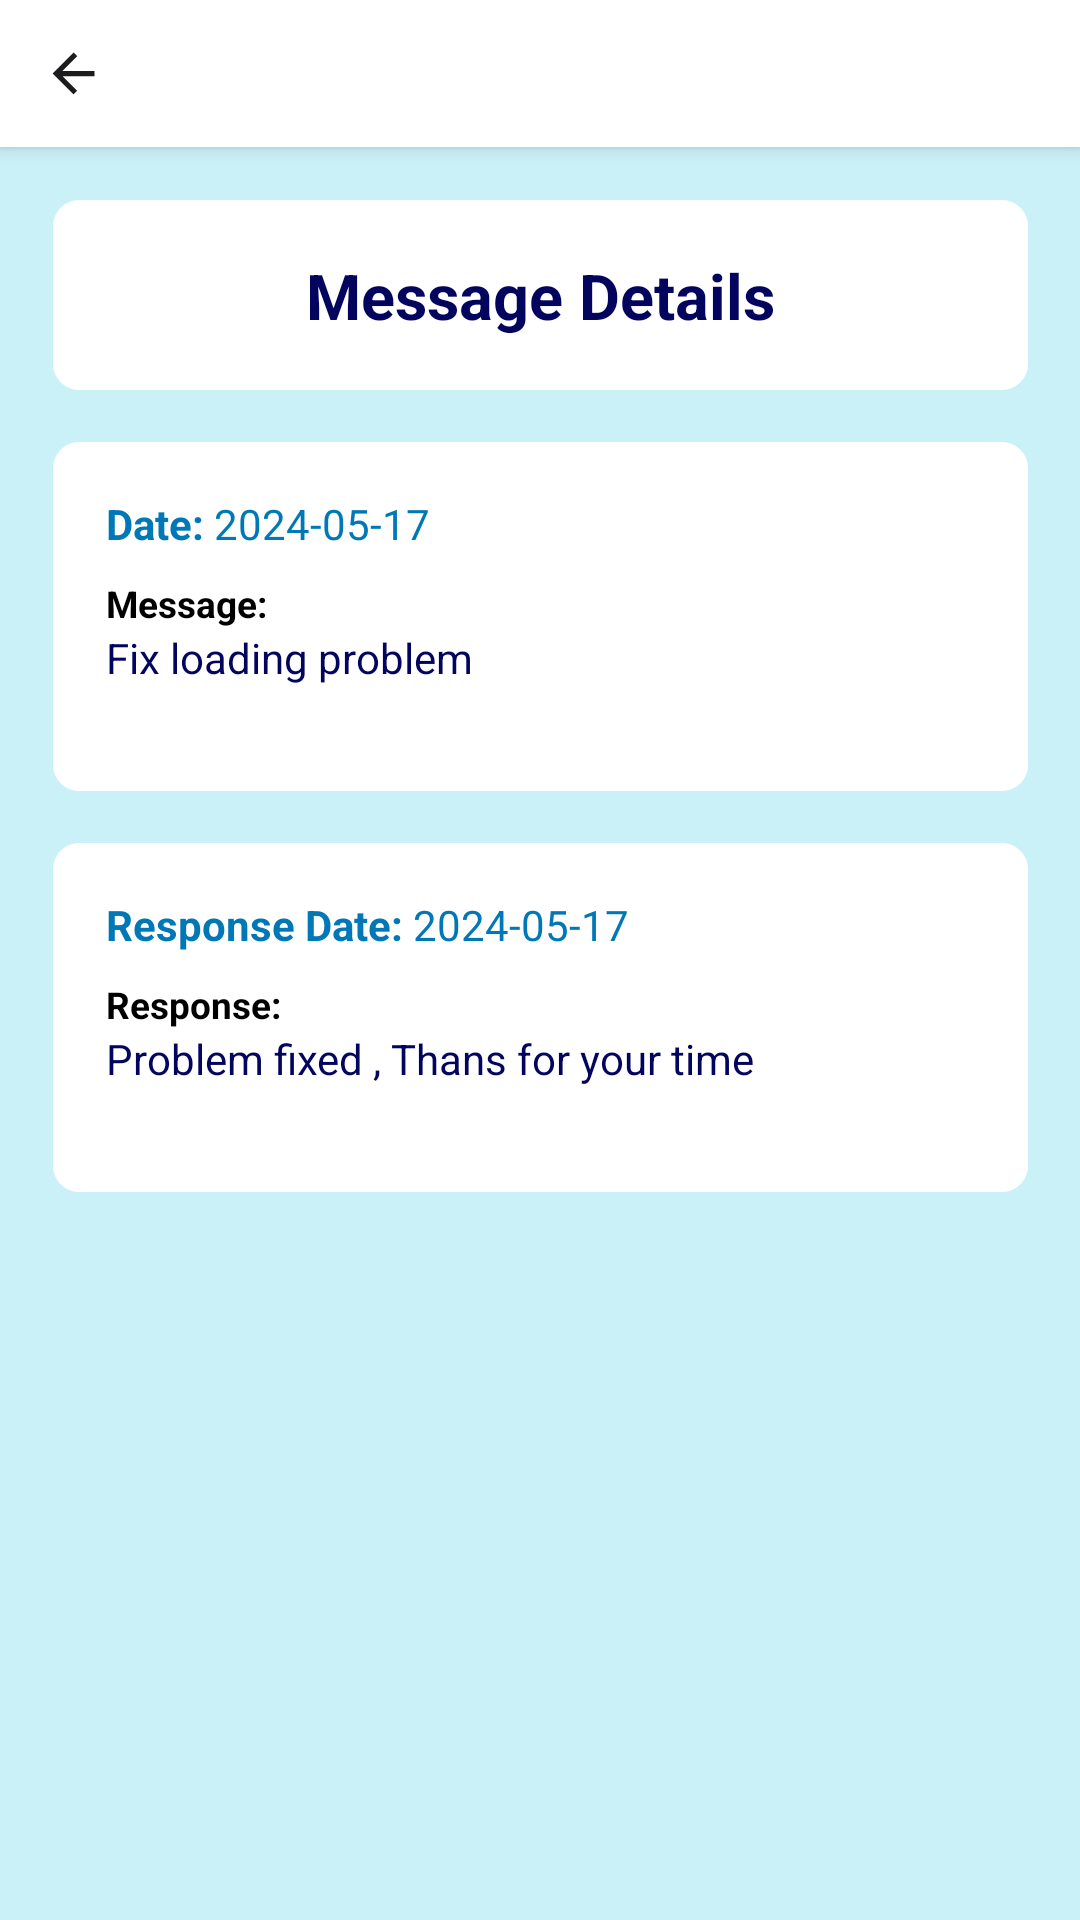
\includegraphics[width=\linewidth]{images/sprint4/feedBackModule (3).png}
    % \caption{Forget Password Sequence Diagram Part 1}
    \label{fig:login-form}
\end{minipage}\hfill
    \caption{Message center Screenshots}
\end{figure}


\section*{Conclusion}

Successfully implementing the "Feedback \& Reviews" module, we have tackled the last major challenge of our project. This feature empowers us to gather critical user feedback, driving continuous enhancement of our app. This milestone marks the completion of our core development phases.
